% ===== 第一部分：单变量分析学 / 第6章：函数的极限与连续性 =====
% !TEX root = ../../main.tex
\setchapterimage{figure/chapter6封面图.png}
\setchapterintro{本章将进入初等分析学中的重点内容——连续性的学习。为了理解连续性，章节首先从函数极限入手，建立函数在一点附近、无穷远处以及左右趋近时的极限概念，再进一步讨论极限的性质，为后面正式研究函数的连续性打基础。
	
	可以概括为一句话：
	
	本章以函数极限为起点，引出并铺垫连续性的学习，这是初等分析学中的核心主题之一。}
\chapter{函数的极限与连续性}
% 第1节：函数极限
% !TEX root = ../../../main.tex
% 所属：第一部分：单变量分析学 / 第6章：函数的极限与连续性
% 节：6.1 函数极限
% 正文按原文件顺序保存；由 ../chapter6.tex 调用。
\section{函数极限}
\begin{definition}\label{def1}
	设函数 $f$ 在点 $x_0$ 的某个去心邻域上有定义，即 $\exists \rho > 0$，使得
	
	$$
	O(x_0, \rho) \setminus \{x_0\} \subset D_f
	$$
	
	对 $A \in \mathbb{R},\text{若} \forall \varepsilon > 0, \exists \delta = \delta(\varepsilon) $ 且 $\delta < \rho$，使得 $\forall x$ 满足 $0 < |x - x_0| < \delta$ 时，
	
	$$
	|f(x) - A| < \eps
	$$
	
	成立，则称 $A$ 为 $f(x)$ 在 $x_0$ 处的极限，记作
	
	$$
	\lim_{x \to x_0} f(x) = A
	$$
	
	若这样的 $A$ 不存在，我们说 $\lim\limits_{x \to x_0} f(x)$ 不存在.
\end{definition}
下面给出 $f(x)$ 在 $x_0$ 的极限不为 $A$ 的定义，这在证明中是经常用的到的.
\begin{definition}\label{nopro}
	$\exists \varepsilon_0 > 0, \forall \delta > 0$，对 $x$，尽管 $0 < |x - x_0| < \delta$，
	
	$$
	|f(x) - A| \geqslant \varepsilon_0
	$$
\end{definition}
接下来我们对极限的定义做出扩展，对$x$的行为以及$f(x)$的行为做出分类，$x$的行为有6种，$f(x)$的行为有4种，两两组合下我们可以得到24种不同极限的定义.

\begin{definition}
	$x$ 的行为：
	
	\begin{enumerate}
		\item $x \to x_0$:~ ————，$\exists \delta > 0, \forall x (0 < |x - x_0| < \delta)$，————
		\item $x \to x_0^+$: ————，$\exists \delta > 0, \forall x (0 < x - x_0 < \delta)$，————
		\item $x \to x_0^-$: ————，$\exists \delta > 0, \forall x (-\delta < x - x_0 < 0)$，————
		\item $x \to \infty$:~~————， $\exists X > 0, \forall x (|x| > X)$，————
		\item $x \to +\infty$: ————，$\exists X > 0, \forall x (x > X)$，————
		\item $x \to -\infty$: ————，$\exists X > 0, \forall x (x < -X)$，————
	\end{enumerate}
	
	其中2、3条与分别对应$x$趋近于$x_0$的左极限与右极限.对函数$f(x)$，$x_0$处 的左右极限记为$f(x_0-),f(x_0+)$
	
	$f(x)$的行为：
	
	\begin{enumerate}
		\item $f(x) \to A$ (有限): $\forall \varepsilon > 0$，————，$  |f(x) - A| < \varepsilon$
		\item $f(x) \to \infty$: $\forall G > 0$，————，$|f(x)| > G$
		\item $f(x) \to +\infty$: $\forall G > 0$，————，$ f(x) > G$
		\item $f(x) \to -\infty$: $\forall G > 0$，————，$ f(x) < -G$
	\end{enumerate}
\end{definition}
举例来说，

$\lim\limits_{x \to x_0} f(x) = \infty$ 定义为

$\forall G > 0, \exists \delta > 0, \forall x$ 满足 $-\delta < x - x_0 < 0$ 有 $|f(x)| > G$ 成立.

$\lim\limits_{x \to +\infty} f(x) = A$ 定义为：

$\forall \varepsilon > 0, \exists X > 0, \forall x$ 满足 $x > X$ 有 $|f(x) - A| < \varepsilon$ 成立.

使用\ref{nopro}中取逆命题的技巧，我们得到一些不收敛于某值，不是无穷的定义

下面给出几个使用定义证明极限的例子.

\begin{example}
	(1)  $$\lim_{x \to 0} e^x = 1$$
	(2)$$\lim_{x \to 1} \frac{x(x-1)}{x^2-1} = \frac{1}{2}$$
	(3)$$\lim_{x \to 1^-} \frac{x^2}{x-1} = -\infty$$
	(4) $$\lim_{x \to \infty} \frac{x+1}{2x-1} = \frac{1}{2}$$
\end{example}
\begin{proof}
	(1) $\forall \varepsilon > 0$，考虑
	\[
	|e^x - 1| < \varepsilon
	\]
	不妨设 $\varepsilon < 1$，
	\[
	1 - \varepsilon < e^x < 1 + \varepsilon
	\]
	取对数得
	\[
	\ln(1 - \varepsilon) < x < \ln(1 + \varepsilon)
	\]
	取 $\delta = \min\{-\ln(1 - \eps), \ln(1 + \eps)\}$，$\forall |x| < \delta$ 都有
	\[
	|e^x - 1| < \varepsilon
	\]
	(2) $\forall \varepsilon > 0$，考虑
	$$\begin{aligned}
		\left|\dfrac{x(x-1)}{x^2-1} - \dfrac{1}{2}\right| &< \varepsilon\\
		\Rightarrow \left|\dfrac{\dfrac{1}{2}(x-1)^2}{x^2-1}\right| &< \eps\\
		\Rightarrow \left|\dfrac{x-1}{2(x+1)}\right| &< \eps
	\end{aligned}$$
	取 $|x-1| < 1$，此时有 $0 < x < 2$，那么 $1 < x+1 < 3$，
	\[
	\left|\dfrac{x-1}{2(x+1)}\right| < \left|\dfrac{x-1}{2}\right| < \eps
	\]
	取 $\delta = \min\{1, 2\varepsilon\}$，$\forall 0 < |x-1| < \delta$ 都有
	\[
	\left|\dfrac{x(x-1)}{x^2-1} - \dfrac{1}{2}\right| < \varepsilon
	\]
	(3) $\forall G > 0$，考虑
	\[
	\frac{x^2}{x-1} < -G
	\]
	取 $-1 < x-1 < 0$，即 $x^2 > 4$，则
	\[
	\frac{x^2}{x-1} < \frac{4}{x-1} < -G
	\]
	取 $\delta = \min\{1, \dfrac{4}{G}\}$，则 $\forall -\delta < x-1 < 0$ 都有
	\[
	\frac{x^2}{x-1} < -G
	\]
	(4) $\forall \varepsilon > 0$，考虑
	$$\begin{aligned}
		\left|\frac{x+1}{2x-1} - \frac{1}{2}\right| &< \varepsilon\\
		\Rightarrow \left|\frac{3}{2(2x-1)}\right| &< \varepsilon
	\end{aligned}$$
	取 $X = \max\left\{\dfrac{3}{4\varepsilon} + \dfrac{1}{2}, \dfrac{3}{-4\varepsilon} - \dfrac{1}{2}\right\}$，$\forall |x| > X$ 都有
	\[
	\left|\frac{x+1}{2x-1} - \frac{1}{2}\right| < \epsilon
	\]
\end{proof}
根据左极限右极限的定义，容易得到以下命题
\begin{proposition}
	$\lim\limits_{x \to x_0} f(x)$ 存在的充要条件是 $f(x)$ 在 $x_0$ 处的左极限、右极限存在并且相等，也就是说：
	\[
	\lim_{x \to x_0} f(x) = A \iff \lim_{x \to x_0^-} f(x) = \lim_{x \to x_0^+} f(x) = A
	\]
\end{proposition}
%
% 第2节：函数极限的性质
% !TEX root = ../../../main.tex
% 所属：第一部分：单变量分析学 / 第6章：函数的极限与连续性
% 节：6.2 函数极限的性质
% 正文按原文件顺序保存；由 ../chapter6.tex 调用。
\section{函数极限的性质}
下面我们叙述函数极限的性质，我们以\ref{def1}中定义的函数极限为例，而其他的23种极限，在有定义的条件下，可以认为下面的性质同样具备.

\begin{proposition}
	设 $A$ 与 $B$ 都是 $f(x)$ 在 $x_0$ 处的极限，即 $A = B$；换句话说，$f(x)$ 在该点的极限唯一.
\end{proposition}
\begin{proof}
	对 $A$ 与 $B$，由极限的定义，
	$$\begin{aligned}
		\forall \varepsilon > 0, &\exists \delta_1 > 0, \forall x (0 < |x - x_0| < \delta_1): |f(x) - A| < \varepsilon\\
		&\exists \delta_2 > 0, \forall x (0 < |x - x_0| < \delta_2): |f(x) - B| < \varepsilon
	\end{aligned}$$
	取 $\delta = \min\{\delta_1,\delta_2\}$，当 $0 < |x - x_0| < \delta$ 时，
	\[
	|A - B| \leqslant |f(x) - A| + |f(x) - B| < 2\varepsilon
	\]
	因为 $\varepsilon$ 是任意的，所以 $|A - B| = 0$，即 $A = B$.
\end{proof}
函数极限有与数列极限相同 的一条性质(\ref{数列的保序性}).

\begin{proposition}
	设 $\lim\limits_{x \to x_0} f(x) = A$，$\lim\limits_{x \to x_0} g(x) = B$，
	
	若 $A > B$，那么存在 $\delta > 0$，使 $0 < |x - x_0| < \delta$ 时，成立 $f(x) > g(x)$.
	\label{partlimits}
\end{proposition}
\begin{proof}
	$$\begin{aligned}
		\forall \varepsilon > 0,&\exists \delta_1 > 0,\forall x (0 < |x - x_0| < \delta_1): |f(x) - A| < \varepsilon\\
		&\exists \delta_2 > 0,\forall x (0 < |x - x_0| < \delta_2): |g(x) - B| < \varepsilon
	\end{aligned}$$
	取 $\delta = \min\{\delta_1, \delta_2\}$，当 $0 < |x - x_0| < \delta$ 时，以上两式同时成立：
	
	再取 $\varepsilon_0 = \dfrac{A - B}{2}$，$\forall \delta, 0 < |x - x_0| < \delta$：
	
	\[
	g(x) < \frac{A + B}{2} < f(x)
	\]
	
\end{proof}
\begin{corollary}
	1. 若 $\lim\limits_{x \to x_0} f(x) = A \neq 0$，则存在 $\delta > 0$，当 $0 < |x - x_0| < \delta$ 时成立
	\[
	|f(x)| > \frac{|A|}{2}
	\]
	
	2. 若 $\lim\limits_{x \to x_0} f(x) = A$，$\lim\limits_{x \to x_0} g(x) = B$，且 $\exists r > 0$，使 $\forall x (0 < |x - x_0| < r)$ 成立 $g(x) \leqslant f(x)$，则 $B \leqslant A$
\end{corollary}
\begin{proof}
	1. 取 \ref{partlimits}中 $f(x) \Rightarrow |f(x)|$，$g(x) \Rightarrow \dfrac{|A|}{2}$，成立.
	
	2. 若不然，则 $B > A$，由 \ref{partlimits}，$\exists \delta > 0$，$\forall x (0 < |x - x_0| < \delta)$ 成立 $f(x) < g(x)$，
	取 $\eta = \min\{\delta, r\}$，当 $0 < |x - x_0| < \eta$ 时，$f(x) < g(x)$ 与 $g(x) \leqslant f(x)$ 矛盾.
	
\end{proof}
\begin{proposition}
	若 $\lim\limits_{x \to x_0} f(x) = A\in\R$，则存在 $\delta > 0$，使得 $f(x)$ 在 $O(x_0, \delta) \setminus \{x_0\}$ 中有界.
\end{proposition}
\begin{proof}
	取 $\varepsilon = 1$，$\exists \delta > 0$，使 $0 < |x - x_0| < \delta$ 时，$|f(x) - A| < \varepsilon = 1$，
	
	即有
	\[
	A - 1 < f(x) < A + 1 \implies |f(x)| < |A| + 1
	\]
	
	即有界.
\end{proof}
\begin{proposition}
	若存在 $r > 0$，使 $\forall x (0 < |x - x_0| < r)$ 成立 $g(x) \leqslant f(x) \leqslant h(x)$，
	
	且 $\lim\limits_{x \to x_0} g(x) = \lim\limits_{x \to x_0} h(x) = A$，则 $\lim\limits_{x \to x_0} f(x) = A$.
\end{proposition}
\begin{proof}
	$$\begin{aligned}
		\forall \varepsilon > 0,&\exists 0 < \delta_1 < r,\forall x (0 < |x - x_0| < \delta_1): A - \varepsilon < g(x)\\
		&\exists 0 < \delta_2 < r,\forall x (0 < |x - x_0| < \delta_2): h(x) < A + \varepsilon
	\end{aligned}$$
	取 $\delta = \min\{\delta_1, \delta_2\}$，当 $0 < |x - x_0| < \delta$，
	\[
	A - \varepsilon < g(x) \leqslant f(x) <h(x) < A + \varepsilon
	\]
	即
	\[
	|f(x) - A| < \varepsilon
	\]
	$\forall x: 0 < |x - x_0| < \delta$
	\[
	\lim_{x \to x_0} f(x) = A
	\]
\end{proof}
\begin{proposition}
	$$\lim_{x\to0}\frac{\sin x}{x}=1$$
\end{proposition}
\begin{proof}
	$x\to0$且$\dfrac{\sin(-x)}{-x}=\dfrac{\sin x}{x}$，不妨设$0<x<\dfrac{\pi}{2}$
	
	考虑下图
	\begin{center}
		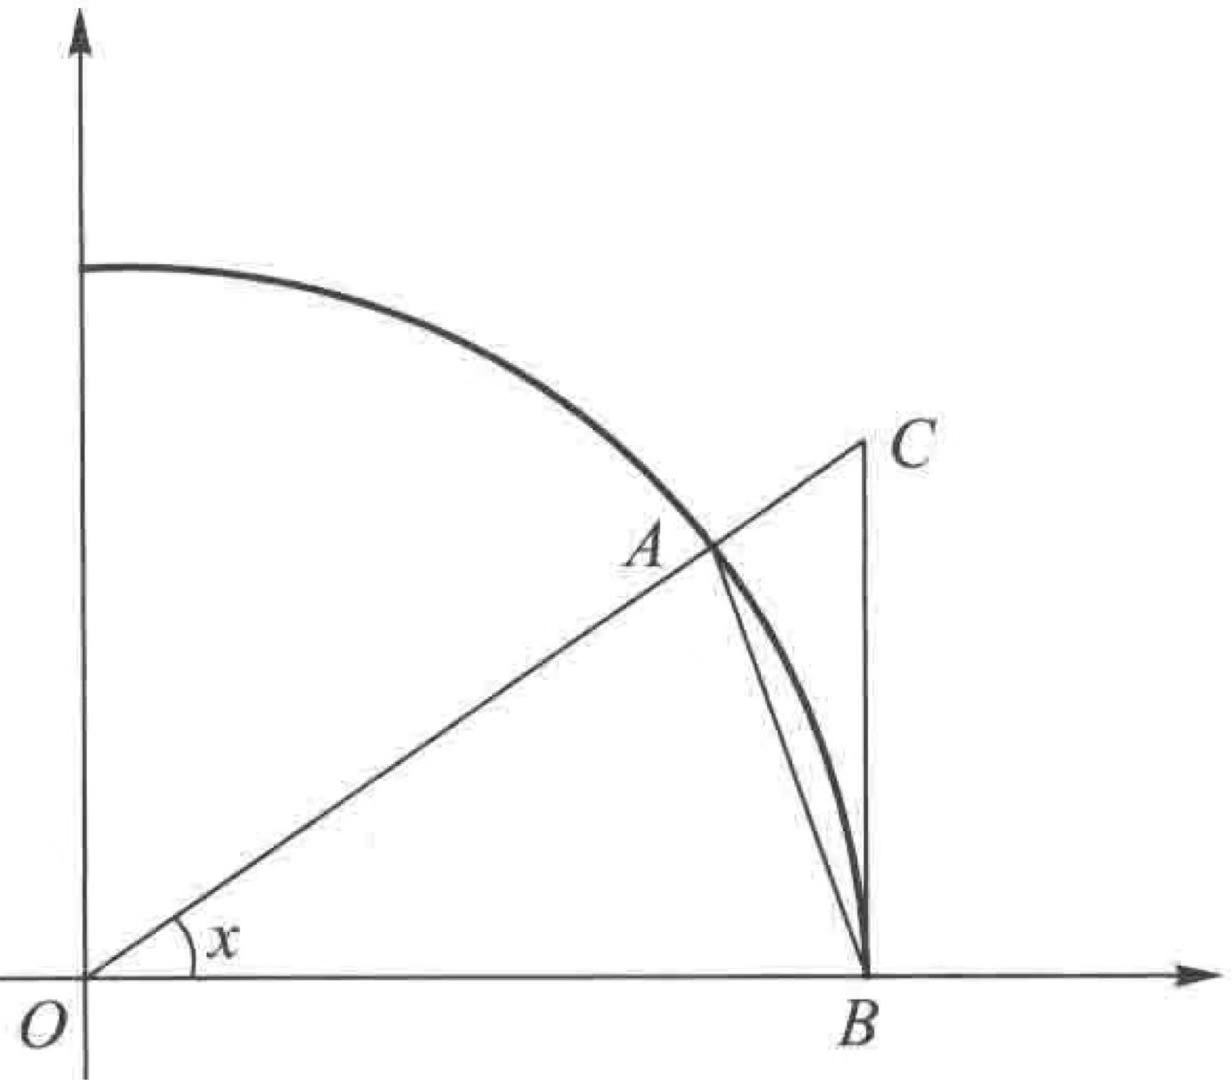
\includegraphics[width=0.3\linewidth]{figure/C5/1}
	\end{center}
	设
	\[
	S_{\triangle OAB} = \frac{1}{2} \sin x = S_1
	\]
	\[
	S_{\triangle OAC} = \frac{1}{2} \tan x = S_2
	\]
	\[
	S_{\textbf{扇形}OAB} = \frac{1}{2} x = S_3
	\]
	
	显然地，
	\[
	S_1 < S_3 < S_2
	\]
	
	也即
	\[
	\sin x < x < \tan x 
	\]
	由于$ x \in \left(0, \dfrac{\pi}{2}\right)$
	\[\frac{\sin x}{x}<1<\frac{\tan x}{x}\Leftrightarrow\cos x<\frac{\sin x}{x}<1\quad x\in(0,\frac{\pi}{2})\]
	下证 $\lim\limits_{x \to 0} \cos x = 1$，也即证明 $f(x) = \cos x$ 在 $x = 0$ 处的连续性.
	
	$\forall \varepsilon > 0$，考虑
	
	\[
	|\cos x - 1| = 2 \sin^2 \frac{x}{2} < \frac{x^2}{2} < \varepsilon
	\]
	
	取 $\delta = \min\left\{\dfrac{\pi}{2}, \sqrt{2\eps}\right\}$，则 $\lim\limits_{x \to 0} \cos x = 1$ 得证.
	
	综上，
	\[
	\lim_{x \to 0} \frac{\sin x}{x} = 1
	\]
\end{proof}
\begin{proposition}
	设 $\lim\limits_{x \to x_0} f(x) = A$，$\lim\limits_{x \to x_0} g(x) = B$，则：
	
	(1) $$\lim_{x \to x_0} (\alpha f(x) + \beta g(x)) = \alpha A + \beta B$$
	
	(2) $$\lim_{x \to x_0} f(x)g(x) = AB$$
	
	(3) $$\lim_{x \to x_0} \frac{f(x)}{g(x)} = \frac{A}{B}\quad B \neq 0$$ 
	
\end{proposition}
\begin{proof}
	$$\begin{aligned}
		\forall \varepsilon > 0,&\exists \delta_1 > 0,\forall x (0 < |x - x_0| < \delta_1): |f(x) - A| < \varepsilon\\
		&\exists \delta_2 > 0,\forall x (0 < |x - x_0| < \delta_2): |g(x) - B| < \varepsilon
	\end{aligned}$$
	
	取 $0 < |x - x_0| < \min\{\delta_1, \delta_2\}$，则两式同时成立.
	
	由有界性：$\forall 0 < |x - x_0| < \min\{\delta_1, \delta_2\}$，$\exists M$，使 $|f(x)| \leqslant M$，$|g(x)| \leqslant M$.
	
	(1)	取 $0 < |x - x_0| < \min\{\delta_1, \delta_2\}$
	\[
	|\alpha f(x) + \beta g(x) - (\alpha A + \beta B)| \leqslant |\alpha||f(x) - A| + |\beta||g(x) - B| < 2\varepsilon
	\]
	
	(2) 取 $0 < |x - x_0| < \min\{\delta_1, \delta_2\}$，
	$$\begin{aligned}
		|f(x)g(x) - AB| &= |f(x)g(x) - g(x)A + g(x)A - AB|\\ 
		&< M|f(x) - A| + |A||g(x) - B| < (M + |A|)\varepsilon
	\end{aligned}$$
	
	
	(3) 取 $0 < |x - x_0| < \min\{\delta_1, \delta_2\}$，
	\[
	\left|\frac{f(x)}{g(x)} - \frac{A}{B}\right| = \left|\frac{Bf(x) - BA + BA - Ag(x)}{Bg(x)}\right| < \frac{2(|A| + |B|)}{B^2} \varepsilon
	\]
	
\end{proof}
\begin{theorem}(Heine定理)\label{Heine1}
	$\lim\limits_{x \to x_0} f(x) = A~\Leftrightarrow~$ $\forall \{x_n\}$ 满足 $x_n \in O(x_0, \rho) \setminus \{x_0\}$ 对某$\rho$，且 $\lim\limits_{n \to \infty} x_n = x_0$，数列 $\{f(x_n)\}$ 满足 $\lim\limits_{n \to \infty} f(x_n) = A$.
\end{theorem}
\begin{proof}
	$\Rightarrow$ 若 $f(x) \to A$ 当 $x \to x_0$，
	
	$\forall \varepsilon > 0, \exists \delta > 0, \forall x (0 < |x - x_0| < \delta): |f(x) - A| < \varepsilon(*)$
	
	由 $x_n \to x_0$，对上述 $\delta > 0, \exists N, \forall n > N$ 
	\[
	0 < |x_n - x_0| < \delta
	\]
	
	由 $(*)$， 因$ x_n \in O(x_0, \rho) \setminus \{x_0\}$，那么 $ |f(x_n) - A| < \varepsilon$
	
	综上$\forall \varepsilon > 0, \exists N, \forall n > N, |f(x_n) - A| < \varepsilon$
	
	$\Leftarrow$ 若不然，$\lim\limits_{x\to x_0}f(x)\neq A$
	
	$\exists \eps_0>0,\forall \delta>0,\exists \widetilde{x},~$即使$0<|\widetilde{x}-x_0|<\delta$，亦有$|f(\widetilde{x})-A|\geqslant\eps_0$
	
	取 $\delta_1 = 1, \exists x_1 (0 < |x_1 - x_0| < \delta_1): |f(x_1) - A| \geqslant \varepsilon_0$，
	
	取 $\delta_2 = \dfrac{1}{2}, \exists x_2 (0 < |x_2 - x_0| < \delta_2): |f(x_2) - A| \geqslant \varepsilon_0$，
	
	$\cdots$
	
	取 $\delta_k = \dfrac{1}{k}, \exists x_k (0 < |x_k - x_0| < \delta_k): |f(x_k) - A| \geqslant \varepsilon_0$，
	
	$\cdots$
	
	这样，我们得到一个列 $\{x_n\}$ 满足 $0 < |x_n - x_0| < \dfrac{1}{n}$ 且 $\lim\limits_{n \to \infty} x_n = x_0$，但是 $|f(x_n) - A| \geqslant \varepsilon_0$，矛盾.
\end{proof}
\begin{corollary}
	(Heine定理的等价叙述)
	$\lim\limits_{x \to x_0} f(x)$ 存在且有限$\Leftrightarrow$对任意序列 $\{x_n\}, x_n \in O(x_0, \rho) \setminus \{x_0\}$ 且 $x_n \to x_0$，$\lim\limits_{n \to \infty} f(x_n)$ 存在且有限.
	
\end{corollary}

\begin{proof}
	必要性$(\Rightarrow)$:同\ref{Heine1}的必要性证明
	
	充分性$(\Leftarrow)$:
	由\ref{Heine1}，只需对任意序列 $\{x_n\}$，$\{f(x_n)\}$ 收敛于同一极限.
	
	如若不然，设 $\{x_n'\}$ 满足 $x_n' \to x_0$，且 $f(x_n') \to A$;$\{x''_n\}$ 满足 $x''_n \to x_0$，且 $f(x''_n) \to B$.
	
	构造数列 $\{x_n\}$ 令 $x_{2n-1} = x_n'$，$x_{2n} = x''_n$，则 $x_n \to x_0$，但 $f(x_n)$ 不收敛，矛盾.
\end{proof}
\begin{example}
	(1) 考虑 $f(x) = \dfrac{a_n x^n + \cdots + a_k x^k}{b_m x^m + \cdots + b_j x^j}$ 在 $x \to 0$ 或 $x \to \infty$ 处的极限.
	
	(2) 证明
	\[
	\lim_{x \to \infty} \left(1 + \frac{1}{x}\right)^x = e
	\]
	
	(3) 证明
	\[
	\lim_{x \to 0} \sin \frac{1}{x} \text{ 不存在}
	\]
\end{example}
\begin{proof}
	(1)
	\[
	\lim_{x \to 0} f(x) =
	\begin{cases}
		\dfrac{a_k}{b_k}, & k = j, \\
		0, & k > j, \\
		\infty, & k < j.
	\end{cases}
	\]
	
	\[
	\lim_{x \to \infty} f(x) =
	\begin{cases}
		\dfrac{a_n}{b_m}, & n = m, \\
		0, & n < m, \\
		\infty, & n > m.
	\end{cases}
	\]
	(2)先考虑$\lim\limits_{x\to+\infty}(1+\dfrac{1}{x})^x$
	
	$\forall x \geqslant 1$，
	\[
	\left(1 + \frac{1}{\lfloor x \rfloor}\right)^{\lfloor x \rfloor} < \left(1 + \frac{1}{x}\right)^x < \left(1 + \frac{1}{\lfloor x \rfloor + 1}\right)^{\lfloor x \rfloor + 1}
	\]
	
	对上式左右两取极限，等价于下式，
	\[
	\lim_{n \to \infty} \left(1 + \frac{1}{n+1}\right)^{n} = e \quad \text{且} \quad \lim_{n \to \infty} \left(1 + \frac{1}{n}\right)^{n+1} = e
	\]
	由夹逼性，
	\[
	\lim_{x \to +\infty} \left(1 + \frac{1}{x}\right)^x = e
	\]
	考虑 $x \to -\infty$ 的情况，令 $y = -x$，$y \to +\infty$，则
	\[
	\lim_{x \to -\infty} \left(1 + \frac{1}{x}\right)^x = \lim_{y \to +\infty} \left(1 - \frac{1}{y}\right)^{-y} = \lim_{y \to +\infty} \left[\left(1 + \frac{1}{y-1}\right)^{y-1} \cdot \left(1 + \frac{1}{y-1}\right)\right] = e
	\]
	综上，
	\[
	\lim_{x \to \infty} \left(1 + \frac{1}{x}\right)^x = e
	\]
	(3) 取 $x_n^{(1)} = \dfrac{1}{n\pi}$，$x_n^{(2)} = \dfrac{1}{2n\pi + \dfrac{\pi}{2}}$，其中 $n = 1, 2, 3, \ldots$
	
	那么 $\lim\limits_{n \to \infty} x_n^{(1)} = \lim\limits_{n \to \infty} x_n^{(2)} = 0$，而 
	$$\lim_{n \to \infty} \sin \frac{1}{x_n^{(1)}} = \lim_{n \to \infty} \sin n\pi = 0,\lim_{n \to \infty} \sin \frac{1}{x_n^{(2)}} = \lim_{n \to \infty} \sin \left(2n\pi + \frac{\pi}{2}\right) = 1$$
	
	由 Heine 定理，$\lim\limits_{x \to 0} \sin \dfrac{1}{x}$ 不存在.
\end{proof}
\begin{proposition}
	(函数极限的Cauchy收敛原理)
	$\lim\limits_{x\to x_0}f(x)$存在且有限
	
	$\Leftrightarrow\forall \varepsilon > 0, \exists \delta > 0, \forall x', x'' \in O(x_0, \delta)\setminus\{x_0\}, |f(x') - f(x'')| < \varepsilon$
	\label{cauchyoffun}
\end{proposition}

\begin{proof}
	$\Rightarrow$:设$\lim\limits_{x \to x_0} f(x) = A$，那么 $\forall \varepsilon > 0, \exists \delta > 0, \forall x', x'' \in O(x_0, \delta) \setminus \{x_0\}$ 都有 $|f(x') - A| < \varepsilon$ 与 $|f(x'') - A| < \varepsilon$.
	
	那么
	\[
	|f(x') - f(x'')| < |f(x') - A| + |f(x'') - A| < 2\varepsilon
	\]
	
	$\Leftarrow$:已知$\forall \varepsilon > 0, \exists \delta > 0, \forall x',x'' \in O(x_0, \delta) \setminus\{x_0\}$ 有 $|f(x') - f(x'')| < \varepsilon$.
	
	$\forall \{x_n\}$使得$\{f(x_n)\}$有定义，且收敛于 $x_0$，对上述的 $\delta$，有
	$$\begin{aligned}
		\exists N, &\forall n > N,\textbf{有} |x_n - x_0| < \delta\\
		&\forall p > 0,\textbf{有} |x_{n+p} - x_0| < \delta
	\end{aligned}$$
	那么
	\[
	|f(x_n) - f(x_{n+p})| < \varepsilon
	\]
	
	因此 $\{f(x_n)\}$ 是 Cauchy 列，所以 $\{f(x_n)\}$ 收敛，由 Heine 定理，$\lim\limits_{x \to x_0} f(x)$ 存在且有极限
	
\end{proof}
注意：对24种不同的极限，在有定义 的情况下都有相应的Cauchy收敛原理，相应的证法各有不同，下举一例

\begin{example}
	$\lim\limits_{x \to +\infty} f(x)$ 存在且有限
	
	$\Leftrightarrow \forall \varepsilon > 0, \exists X, \text{使得} \, \forall x', x'' > X, \text{都有} \, |f(x') - f(x'')| < \varepsilon$
\end{example}
\begin{proof}
	$\Rightarrow$ 同 \ref{cauchyoffun} ，略
	
	$\Leftarrow$ 已知 $\forall \varepsilon > 0, \exists X > 0, \text{使得} \, \forall x', x'' > X  \text{都有} \, |f(x') - f(x'')| < \varepsilon$.
	
	$\forall \{x_n\}$ 满足 $x_n \to +\infty$，则 $\exists N, \forall n > N, \text{有} \, x_n > X$.
	
	对上述 $X$，$\exists N, \forall n > N, \text{有} \, x_n > X$，$\forall p > 0, \text{有} \, x_{n+p} > X$，则
	\[
	|f(x_n) - f(x_{n+p})| < \varepsilon
	\]
	
	因此，$\{f(x_n)\}$ 是一个 Cauchy 列，则 $\{f(x_n)\}$ 收敛且有界.由 Heine 定理，$\lim\limits_{x \to +\infty} f(x)$ 存在且有限.
\end{proof}

%
% 第3节：连续性
% !TEX root = ../../../main.tex
% 所属：第一部分：单变量分析学 / 第6章：函数的极限与连续性
% 节：6.3 连续性
% 正文按原文件顺序保存；由 ../chapter6.tex 调用。
\section{连续性}
\begin{definition}
	对 函数$f(x)$，若满足：
	\begin{enumerate}
		\item $f(x) $在$ O(x_0, \rho)$ 上有定义，对某 $\rho$(此处无需去心邻域)
		\item $\lim\limits_{x \to x_0} f(x)$ 存在
		\item $\lim\limits_{x \to x_0} f(x) = f(x_0)$
	\end{enumerate}
	
	就说 $f(x)$ 在 $x_0$ 处连续.或等价地，用“$\varepsilon-\delta$”语言：
	
	$f(x) $在$ O(x_0, \rho)$ 上有定义，对某 $\rho$，$\forall \varepsilon > 0$，$\exists \delta(\varepsilon, x_0)> 0$，$\forall x (|x - x_0| < \delta)$：
	\[
	|f(x) - f(x_0)| < \varepsilon
	\]
	
\end{definition}
\begin{definition}
	对 $f(x)$，若：
	\begin{itemize}
		\item $f(x)$ 在 $[x_0, x_0 + \rho)$ 上有定义，且 $\lim\limits_{x \to x_0^+} f(x) = f(x_0)$，则称 $f(x)$ 在$x_0$右连续.
		\item $f(x)$ 在 $(x_0 - \rho, x_0]$ 上有定义，且 $\lim\limits_{x \to x_0^-} f(x) = f(x_0)$，则称 $f(x)$ 在$x_0$左连续.
	\end{itemize}
	显然，若 $f(x)$ 在 $x_0$ 处连续，则必有
	\[
	\lim_{x \to x_0^+} f(x) = \lim_{x \to x_0^-} f(x) = f(x_0)
	\]
\end{definition}

\begin{definition}
	若 $f(x)$ 在开区间 $(a, b)$ 上的任意一点处连续，那么称 $f(x)$ 在开区间 $(a, b)$ 上连续.记为$f\in C(a,b)$.
	
	若 $f(x)$ 在 $(a, b)$ 上连续，同时在 $x = a$ 处右连续，在 $x = b$ 处左连续，那么称 $f(x)$ 在闭区间 $[a, b]$ 上连续.记为$f\in C[a,b]$
	
	
\end{definition}
\begin{proposition}
	
	设 $f(x), g(x)$ 在 $x_0$ 处连续，那么有
	
	(1) $$\lim_{x \to x_0} (\alpha f(x) + \beta g(x)) = \alpha f(x_0) + \beta g(x_0)$$
	
	更一般地，有限个连续函数的线性组合仍连续，而无限个连续函数的“线性组合”未必连续，甚至未必有意义.
	
	(2) $$\lim_{x \to x_0} f(x)g(x) = f(x_0)g(x_0)$$
	
	更一般地，有限个连续函数的乘积仍连续，无限个连续的乘积则未必，甚至未必有定义
	
	(3) $$\lim_{x \to x_0} \frac{f(x)}{g(x)} = \frac{f(x_0)}{g(x_0)}\quad g(x_0) \neq 0$$ 
\end{proposition}
\begin{proof}
	由函数极限的定义的易知
\end{proof}

考虑 $f(x)$ 在 $x_0$ 处连续的定义：
\begin{enumerate}
	\item 在 $x_0$ 处左右极限存在且相等；
	\item 在 1 下，$\lim\limits_{x \to x_0^+} f(x) =\lim\limits_{x \to x_0^-} f(x)= f(x_0)$
\end{enumerate}

逐一的破坏极限的定义，我们得出 $f(x)$在$x_0$ 的三类不连续点的定义.
\begin{definition}
	设 $f(x)$ 在 $x_0$ 的某邻域内有定义
	\begin{enumerate}
		\item  若 $f(x)$ 在 $x_0$ 处的左右极限存在，且 $f(x_0-) \neq f(x_0+)$，则称 $x_0$ 为第一类间断点，又称跳跃间断点（$|f(x_0+) - f(x_0-)|$ 为 $x_0$ 上的跃度）.
		\item 若 $f(x)$ 在 $x_0$ 处的左右极限至少有一不存在，则称 $x_0$ 为第二类间断点.
		\item 若 $f(x)$ 在 $x_0$ 处的左右极限都存在且相等，但 $f(x_0+) = f(x_0-) \neq f(x_0)$，则称 $x_0$ 为第三类间断点.此时，令	
		\[
		\widetilde{f}(x) = \begin{cases}
			f(x) & x \neq x_0 \\
			f(x_0+) = f(x_0-) & x = x_0
		\end{cases}
		\]
	\end{enumerate}
	在 $f$ 无其他不连续点的情况下，$\widetilde{f}(x)$ 是连续的.第三类间断点又称可去间断点.
	
	有些时候，$f$ 在 $x_0$ 处无定义，我们把这种情况也归入第三类间断点
	
	还有一种间断点，顾名思义的，无穷间断点，因各个教材的分类不同，此处单取一类
\end{definition}
我们给出几个例子

\begin{example}
	考虑从下列函数的不连续点以及不连续点的类型：
	
	(1) $f(x) = \dfrac{\sin x}{x}$
	
	(2) $D(x) = \begin{cases}
		1, & x \in \mathbb{Q} \\
		0, & x \in \mathbb{R} \setminus\mathbb{Q}
	\end{cases}$
	
	(3) $R(x) = \begin{cases}
		\dfrac{1}{p}, & x = \dfrac{q}{p}, p\in\Z_+,q\in\Z\setminus\{0\},\text{$p$ 和 $q$ 互质}\\
		1, & x = 0 \\
		0, & x \in \mathbb{R} \setminus \mathbb{Q}
	\end{cases}$
	
	(4) $g(x) = \text{sgn}(x)$
\end{example}
\begin{proof}
	1. 函数 \( f(x) \) 在 \( x = 0 \) 处无定义，但 \(\lim\limits_{x \to 0^+} \dfrac{\sin x}{x} = \lim\limits_{x \to 0^-} \dfrac{\sin x}{x} = 1\)，故 \( x = 0 \) 是第三类间断点；
	
	2. 对 \(\forall x_0 \in \mathbb{R}\)，考虑两个列 $\{x_n\},\{y_n\}$满足 \(x_n \in \mathbb{Q}, y_n \in \mathbb{R} \setminus \mathbb{Q}\)，
	且 \(x_n, y_n < x_0\)，\(x_n, y_n \to x_0\)，那么
	\[
	\lim_{n \to \infty} D(x_n) = 1, \quad \lim_{n \to \infty} D(y_n) = 0
	\]
	
	由 Heine 定理 \(\lim\limits_{x \to x_0} D(x)\) 不存在，即 \(D(x)\) 在 \(x_0\) 处间断.故任意一点都是第二类间断点.
	
	(3) $R(x+1) = R(x)$，故 $R(x)$ 是 1 为周期的函数，只需考虑 $[0,1]$ 这一区间上的点即可.
	
	对任意无理点 $x_0 \in \mathbb{R} \setminus \mathbb{Q}$，对 $R(x_0) = 0$ 且 $\lim\limits_{x \to x_0} R(x) = 0$，故在任意无理点处连续.
	
	下面考虑 $[0,1]$ 上的有理数 $x_0$，下证 $\lim\limits_{x \to x_0} R(x) = 0$.
	
	$\forall \varepsilon > 0$，考虑 $|R(x)| < \varepsilon$，求相应的$\delta$.
	
	反向的考虑：在 $[0,1]$ 的区间里，$R(x) \geqslant \varepsilon$ 的点有多少个.
	
	$\eps>0,\exists n$，使得$\dfrac{1}{10^{n-1}}>\eps\geqslant \dfrac{1}{10^n}$，$R(x)>\dfrac{1}{10^n}$
	
	比如 ,$n=1$ 时，$R(x) = 1, \dfrac{1}{2}, \dots, \dfrac{1}{9}>\dfrac{1}{10}$;$n=2$ 时，$R(x) = 1, \dfrac{1}{2}, \dots, \dfrac{1}{99}>\dfrac{1}{100}$
	
	显然，使 $R(x) > \dfrac{1}{10^n}$ 的有理数 $x \in [0,1]$ 是有限的.设为 $x_1, \dots, x_n$，假设其中不含$x_0$,$\forall1\leqslant k\leqslant n,|x_k - x_0|>0$，取 $\delta= \min\limits_{1 \leqslant k \leqslant n} |x_k - x_0|>0$.则 $0 < |x - x_0| < \delta$ 时，$R(x) < \varepsilon$.
	
	综上 $\lim\limits_{x \to x_0} R(x) = 0$而$R(x_0) = \dfrac{1}{p}$，故在有理点上不连续，属第二类间断点.
	
	(4) 显然，$\lim\limits_{x \to 0^-} \text{sgn}(x) = -1$，$\lim\limits_{x \to 0^+} \text{sgn}(x) = 1$，而 $\text{sgn}(0) = 0$.故 $x = 0$ 为第一类间断点，且跃度为 2.
\end{proof}
\begin{proposition}
	设函数 $f$ 在区间 $(a, b)$ 上单调，那么$(a, b)$ 中使$f$ 间断的点的集是至多可数.
\end{proposition}

\begin{proof}
	设 $E$ 是 $f$ 所有间断点构成的集合，假设$f$是单调递增的.对于 $\forall x \in E$，$\exists r \in \mathbb{Q},r=r(x)$，使得 $f(x-) < r(x) < f(x+)$.
	
	由 $x_1 < x_2$，若 $f(x_1+) \leqslant f(x_2-)$，所以$x_1 \neq x_2$ 时，$r(x_1) \neq r(x_2)$.
	
	因此，在 $E$ 与 $\mathbb{Q}$ 的子集上建立了一一对应.
\end{proof}
\begin{proposition}
	$(a, b)$ 上的单调函数(未必严格单调)的不连续点必为第一类间断点.
	\label{monouni}
	
\end{proposition}
\begin{proof}
	不妨设函数 $f(x)$ 单调上升，
	
	令 $S = \{ f(x): x \in (a, x_0) \}$.
	
	因 $f\left(\dfrac{x_0 + a}{2}\right) \in S$ 故 $S \neq \varnothing$ 且有上界（$f(x_0)$ 是 $S$ 的一个上界）.
	
	那么，由确界原理 $\beta = \sup S$ 存在.
	
	对 $\beta = \sup S$，$\forall \varepsilon > 0$，$\exists x^* \in (a, x_0)$，使 $f(x^*) > \beta - \varepsilon$.
	
	取 $\delta = x_0 - x^* > 0$，当 $x \in (x_0 - \delta, x_0)$，$x^* < x < x_0$，
	
	$$\beta - \varepsilon < f(x^*) \leqslant f(x) \leqslant \beta \Leftrightarrow-\eps<f(x)-\beta\leqslant0$$
	
	因此 $f(x_0-)$ 存在，同理 $f(x_0+)$存在.
\end{proof}
下面我们考虑连续性之于反函数
\begin{proposition}\label{infunex}
	证明：$f(x)$ 在 $D_f \subset \mathbb{R}$ 上严格单调增（或严格单调减），则 $y = f(x)$ 的反函数 $x = f^{-1}(y)$：$R_f \to D_f$ 存在，且 $f^{-1}(y)$ 也为严格单调增（或严格单调减）.
	
\end{proposition}
\begin{proof}
	
	存在性：由 $f$ 是严格单调，$f^{-1}$ 满足映射定义一 对一的条件，存在性得证.
	
	单调性：设 $f$ 是严格单调增，
	若 $f^{-1}$ 不严格单调增，则$f^{-1}$为单调减，那么 $\forall y_1, y_2 \in R_f$，设 $y_1 < y_2$，但 $x_1 = f^{-1}(y_1) \geqslant x_2 = f^{-1}(y_2)$，又因 $f$ 单增，$x_1 \geqslant x_2$，$f(x_1) \geqslant f(x_2)$ 矛盾.
	
\end{proof}
\begin{proposition}
	设函数 $y = f(x)$ 在闭区间 $[a, b]$ 上连续且严格单调增，$f(a) = \alpha$，$f(b) = \beta$，则其反函数 $x = f^{-1}(y)$ 在 $[\alpha, \beta]$ 上连续且严格单调增.
	
	
\end{proposition}
\begin{proof}
	先证$\forall y_0 \in [\alpha, \beta]$，$\exists x_0 \in [a, b]$，使得 $f(x_0) = y_0$，换言之$$f([a, b]) = [\alpha, \beta]$$
	
	设 $\gamma \in (\alpha, \beta)$，设
	$$S = \{x : x \in [a, b], f(x) < \gamma
	\}$$
	由$a\in S$,$S$ 非空，且 $f(b) > \gamma$，$S$ 有上界，由确界原理，$\exists x_0 = \sup S$，$x_0 \in (a, b)$.
	由 $f$ 单调递增，$x<x_0$时，$f(x)<\gamma$;$x>x_0$时，$f(x)>\gamma$.由\ref{monouni}
	$$f(x_0-) \leqslant \gamma \leqslant f(x_0+)$$
	而 $f$ 在 $x_0$ 处连续，$f(x_0) =f(x_0+)=f(x_0-)= \gamma$，这样$f$ 的值域是 $[\alpha, \beta]$
	
	由\ref{infunex}，在 $[\alpha, \beta]$ 上存在$f$的反函数$x=f^{-1}(y)$，且 $f^{-1}$ 严格单调增.
	
	下证 $f^{-1}$ 在 $[\alpha, \beta]$ 上的连续性：
	
	设 $y_0 \in (\alpha, \beta)$，相应的有 $f^{-1}(y_0) = x_0 \in (a, b)$.对于任意 $\varepsilon > 0$，找出$\delta > 0$，使得 $|y - y_0| < \delta$ 时，
	有 
	$$|f^{-1}(y)-f^{-1}(y_0)|=|f^{-1}(y)-x_0|<\eps$$
	即$$x_0-\eps<f^{-1}(y)<x_0+\eps$$
	设$y_1 = f(x_0 - \varepsilon),y_2 = f(x_0 + \varepsilon)$
	，令 $\delta = \min\{|y_1 - y_0|, |y_2 - y_0|\}$
	
	$\forall y$ 满足 $|y - y_0| < \delta$，$f^{-1}(y) \in (x_0 - \varepsilon, x_0 + \varepsilon)$，即 $f^{-1}$ 连续.
	
\end{proof}
\begin{proposition}
	设 $u = g(x)$ 在 $x = x_0$ 处连续，$u_0 = g(x_0)$；$y = f(u)$ 在 $u = u_0$ 处连续，则 $y = f \circ g(x)$ 在 $x = x_0$ 处连续，且 $y_0 = f \circ g(x_0)$.
	
	
\end{proposition}
\begin{proof}
	设函数的值域在所讨论的区间中有定义
	
	由 $y = f(u)$ 在 $u = u_0$ 处连续，$\forall \varepsilon > 0$，$\exists \eta > 0$，使 $|u - u_0| < \eta$ 时，
	\[ |f(u) - f(u_0)| < \varepsilon \]
	
	$u = g(x)$ 在 $x = x_0$ 处连续，对上述 $\eta > 0$，$\exists \delta > 0$，使 $|x - x_0| < \delta$ 时，
	\[ |g(x) - g(x_0)| < \eta \Leftrightarrow|u - u_0| < \eta \]
	
	因此，对 $\delta$，$|x-x_0|<\delta$时，
	\[ |f \circ g(x) - f \circ g(x_0)| < \varepsilon \]
	
	即 $f \circ g$ 在 $x = x_0$ 处连续.
\end{proof}
\begin{corollary}
	有限多连续函数的复合依旧是连续的
\end{corollary}
\begin{proof}
	用数学归纳法即可证明
\end{proof}
%
% 第4节：基本初等函数的连续性
% !TEX root = ../../../main.tex
% 所属：第一部分：单变量分析学 / 第6章：函数的极限与连续性
% 节：6.4 基本初等函数的连续性
% 正文按原文件顺序保存；由 ../chapter6.tex 调用。
\section{基本初等函数的连续性}
下面我们考虑各个基本初等函数的连续性.
\begin{proposition}
	显然的，常数函数$f(x)=c(\text{常数})$在定义域上是连续的
\end{proposition}
\begin{proposition}
	$f(x)=x^{\alpha}\quad \alpha\in\R$在定义域上是连续的
\end{proposition}
\begin{proof}
	对 $\alpha \in \mathbb{Z}$，先考虑 $f(x) = x\quad x\in(-\infty, +\infty)$，
	
	$\forall \varepsilon > 0$，取 $\delta = \varepsilon$，$\forall x(0 < |x - x_0| < \delta)$，
	\[ |f(x) - f(x_0)| = |x - x_0| < \varepsilon = \delta \]
	
	$\alpha \in \mathbb{Z}$ 时，$x^\alpha$ 可以看作 $\alpha$ 个 $x$ 的乘积，自然为连续函数
	
	对 $\alpha \in \mathbb{Q}$，先考虑 $f(x) = \sqrt[m]{x}$
	
	$m \in \mathbb{Z}_+$，
	$\forall \varepsilon > 0$，取 $\delta = \varepsilon^m$，$\forall x(0 < |x - x_0| < \delta)$，
	\[ |\sqrt[m]{x} - \sqrt[m]{x_0}| \leqslant\sqrt[m]{|x-x_0|}<\varepsilon \]
	
	$\alpha \in \mathbb{Q}$ ，设 $\alpha = \dfrac{n}{m}$，$f(x) = x^{n/m}$，由复合函数的连续性，对 $\alpha \in \mathbb{Q}$，$x^{\alpha}$在定义域上连续
	
	对 $\alpha \in \mathbb{R} \setminus\mathbb{Q}$，我们之后再说
	
\end{proof}
\begin{proposition}
	函数 $f(x) = a^x$ ($a > 0$, $a \neq 1$) 在 $(-\infty, +\infty)$ 上连续.
\end{proposition}
\begin{proof}
	$\forall x_0 \in (-\infty, +\infty)$，
	\[ a^x - a^{x_0} = a^{x_0}(a^{x - x_0} - 1) \]
	
	因为
	\[ \lim_{x \to x_0} a^x = a^{x_0} \Leftrightarrow \lim_{t \to 0} a^t = 1 \]
	$t \to 0^+$ 时，当 $a > 1$时，有
	\[ 1 < a^t \leqslant a^{1/[\frac{1}{t}]} \]
	而 $\lim\limits_{n \to \infty} a^{1/n} = 1$，由夹逼定理，
	\[ \lim_{t \to 0^+} a^t = 1 \]
	
	$0 < a < 1$ 时，
	\[ \lim_{t \to 0^+} a^t = \lim_{t \to 0^+} \dfrac{1}{\left(\dfrac{1}{a}\right)^t} = 1 \]
	
	$t \to 0^-$ 时，令 $u = -t$，
	\[ \lim_{t \to 0^-} a^t = \lim_{u \to 0^+} a^{-u} = \lim_{u \to 0^+} \frac{1}{a^u} = 1 \]
	
	综上，
	\[ \lim_{t \to 0} a^t = 1 \]
	从而 $\lim\limits_{x \to x_0} a^x = a^{x_0}$.
	
\end{proof}
\begin{corollary}
	$f(x)=\log_a(x)$在定义域上是连续的
\end{corollary}
\begin{proof}
	由$f(x)=a^x$以及反函数连续性定理易得
\end{proof}
\begin{corollary}
	$f(x)=x^{\alpha},\alpha\in\R$在定义域上连续
	
\end{corollary}
\begin{proof}
	$$f(x)=x^{\alpha	}=e^{\alpha\ln x}$$
	由复合函数连续性定理得证
	
\end{proof}
\begin{corollary}
	双曲函数$$\begin{aligned}
		&y=\sinh x &y=\cosh x \quad &y=\tanh x\\
		&y=\mathrm{csch}x &y=\mathrm{sech}x\quad&y=\coth x
	\end{aligned}$$在定义域上是连续的
\end{corollary}
\begin{proposition}
	函数 $f(x) = \sin x$ 与 $g(x) = \cos x$ 在 $(-\infty, +\infty)$ 上连续.
\end{proposition}
\begin{proof}
	对于 $y = \sin x$，$\forall x_0 \in (-\infty, +\infty)$，
	\[
	|\sin x - \sin x_0| = 2 \left|\cos \frac{x_0 + x}{2} \sin \frac{x - x_0}{2}\right| \leqslant |x - x_0|
	\]
	取 $\delta = \varepsilon$，当 $|x - x_0| < \delta$ 时，
	\[
	|\sin x - \sin x_0| < \varepsilon
	\]
	
	对于 $y = \cos x$，$\forall x_0 \in (-\infty, +\infty)$，
	\[
	|\cos x - \cos x_0| = 2 \left|\sin \frac{x_0 + x}{2} \sin \frac{x - x_0}{2}\right| \leqslant |x - x_0|
	\]
	取 $\delta = \varepsilon$，当 $|x - x_0| < \delta$ 时，
	\[
	|\cos x - \cos x_0| < \varepsilon
	\]
	
\end{proof}
\begin{corollary}
	$y=\tan x,y=\cot x,y=\csc x,y=\sec x$在定义域上 是连续的
\end{corollary}

\begin{corollary}
	反三角函数
	\[ y = \sin^{-1} x, \quad y = \cos^{-1} x, \quad y = \tan^{-1} x \]
	\[ y = \csc^{-1} x, \quad y = \sec^{-1} x, \quad y = \cot^{-1} x \]
	在其定义域内连续
\end{corollary}
\begin{corollary}
	基本初等函数的有限次复合函数在其定义域上连续	
\end{corollary}
%
% 第5节：无穷大量与无穷小量的阶
% !TEX root = ../../../main.tex
% 所属：第一部分：单变量分析学 / 第6章：函数的极限与连续性
% 节：6.5 无穷大量与无穷小量的阶
% 正文按原文件顺序保存；由 ../chapter6.tex 调用。
\section{无穷大量与无穷小量的阶}
下面我们介绍阶数这一概念，类似于集合的势的比较，我们定义的阶数揭示了无穷小量趋近于零的相对程度以及无穷大量绝对增长至无穷的相对程度

类似于数列极限中对无穷大量与无穷小量的定义，下面是函数极限中无穷大量与无穷小量 的定义
\begin{definition}
	若 $\lim\limits_{x \to A} f(x) = 0$，则称 $x \to A$ 时 $f(x)$ 是无穷小量.
	
	若 $\lim\limits_{x \to A} f(x) = \infty(\pm\infty
	)$ ，则称 $x \to A$ 时 $f(x)$ 是无穷大量.
	
	这里 $x \to A$ 包括了 $x \to x_0$，$x \to x_0^+$，$x \to x_0^-$，$x \to +\infty$，$x \to -\infty$，$x \to \infty$ 等各种情况，下面用 $x \to x_0$ 举例.
	
\end{definition}
无穷大量与无穷小量的阶定义如下，它是一种相对的定义我们可以说两个无穷量的阶数如何如何，想要给出某一无穷量的绝对阶数，需要与$x^a$做比对
\begin{definition}
	对于 $u(x), v(x)$，当 $x \to x_0$ 时，$u(x), v(x)$ 都是无穷小量.
	
	(1) 若 $\lim\limits_{x \to x_0} \dfrac{u(x)}{v(x)} = 0$，我们称 $x \to x_0$ 时，$u(x)$ 关于 $v(x)$ 是高阶无穷小量或 $v(x)$ 关于 $u(x)$ 是低阶无穷小量，记作
	\[ u(x) = o(v(x)) \quad (x \to x_0). \]
	
	(2) 若 $\exists A > 0$，当$x$ 在$x_0$的某邻域内，成立
	\[ \left| \frac{u(x)}{v(x)} \right| \leqslant A \]
	则称 $x \to x_0$ 时，$\dfrac{u(x)}{v(x)}$ 是有界量，记作
	\[ u(x) = O(v(x)) \quad (x \to x_0). \]
	
	(3) 若 $\exists A\geqslant a > 0$，对于 $x$ 在$x_0$的某去心邻域内，成立
	\[ a \leqslant \left| \frac{u(x)}{v(x)} \right| \leqslant A \]
	则称 $x \to x_0$ 时，$u(x)$ 与 $v(x)$ 是同阶无穷小量.
	
	若 $\lim\limits_{x \to x_0} \dfrac{u(x)}{v(x)} = C \neq 0$，则 $u(x)$ 与 $v(x)$ 必是同阶无穷小量.
	
	(4) 若 $\lim\limits_{x \to x_0} \dfrac{u(x)}{v(x)} = 1$，则称 $x \to x_0$ 时，$u(x)$ 与 $v(x)$ 是等价无穷小量，记作
	\[ u(x) \sim v(x) \quad (x \to x_0). \]
	
	也可以写成
	\[ u(x) = v(x) + o(v(x)) \quad (x \to x_0). \]
	
	表示$x \to x_0$ 时，$u(x)$ 与 $v(x)$ 不一定相等，差一个关于 $v(x)$ 的高阶无穷小量，
	
\end{definition}
\begin{example}
	(1)
	\[
	\lim_{x \to 0} \frac{1 - \cos x}{x} = \lim_{x \to 0} \dfrac{2 \sin^2 \dfrac{x}{2}}{x} = 0
	\]
	所以
	\[
	1 - \cos x = o(x) \quad (x \to 0)
	\]
	
	(2)
	\[
	\lim_{x \to 0} \frac{\tan x - \sin x}{x^2} = \lim_{x \to 0} \left( \frac{\sin x}{x \cos x} \cdot \frac{1 - \cos x}{x} \right) = 0
	\]
	所以
	\[
	\tan x - \sin x = o(x^2) \quad (x \to 0)
	\]
	
	(3)$x \to 0 $时，$x \sin \dfrac{1}{x}$ 是无穷小量，且$\left| \dfrac{x \sin \dfrac{1}{x}}{x} \right| \leqslant 1$，因此 
	\[
	x \sin \frac{1}{x} = O(x) \quad (x \to 0)
	\]
	
	(4)
	\[
	\lim_{x \to 0} \frac{\sin x}{x} = 1
	\]
	所以
	\[
	\sin x \sim x \quad (x \to 0) \quad \text{ 或者 } \quad \sin x = x + o(x) \quad (x \to 0)
	\]
	
	(5)
	\[
	\lim_{x \to 0} \dfrac{1 - \cos x}{\dfrac{1}{2} x^2} = \lim_{x \to 0} \dfrac{2 \sin^2 \dfrac{x}{2}}{\dfrac{1}{2} x^2} = 1
	\]
	所以
	\[
	1 - \cos x \sim \frac{1}{2} x^2 \quad (x \to 0) \quad \text{ 或者 } \quad 1 - \cos x = \frac{1}{2} x^2 + o(x^2) \quad (x \to 0)
	\]
	
	(6)
	\[
	\lim_{x \to 0} \frac{\tan x - \sin x}{\dfrac{1}{2} x^3} = \lim_{x \to 0} \left( \frac{\sin x}{x \cos x} \cdot \dfrac{1 - \cos x}{\dfrac{1}{2} x^2} \right) = 1
	\]
	所以
	\[
	\tan x - \sin x \sim \dfrac{1}{2} x^3 \quad (x \to 0)\text{或者}\tan x - \sin x=\frac{1}{2}x^3+o(x^3)\quad(x\to0)\]
\end{example}
我们往往取 $v(x) = (x - x_0)^k$ 与 $u(x)$ 进行比较 ($x \to x_0$)，若 $x \to \infty$，
则取 $v(x) = \dfrac{1}{x^k}$.我们称 $k$ 为 $u(x)$ 作为无穷小量的阶数.例如
\[ 1 - \cos x \sim \frac{1}{2}x^2 \quad (x \to 0), \]
得 $x \to 0$时，$1 - \cos x$ 是二阶无穷小量.

类似的，对无穷大量我们有类似的定义
\begin{definition}
	对于 $u(x), v(x)$，在 $x \to x_0$ 时，是无穷大量，那么：
	
	(1) 若 $\lim\limits_{x \to x_0} \dfrac{u(x)}{v(x)} = \infty$，则称 $x \to x_0$ 时，$u(x)$ 关于 $v(x)$ 是高阶无穷大量，或 $v(x)$ 关于 $u(x)$ 是低阶无穷大量.
	记作\[v(x)=o(u(x))\]
	(2) 若 $\exists A > 0$，当 $x$ 在 $x_0$ 的某去心邻域中，成立
	\[ \left| \frac{u(x)}{v(x)} \right| \leqslant A \]
	则称 $x \to x_0$ 时，$\dfrac{u(x)}{v(x)}$ 是有界量，记作
	\[ u(x) = O(v(x)) \quad (x \to x_0). \]
	
	(3) 若 $\exists A, a > 0$，当 $x$ 在 $x_0$ 的某去心邻域中，成立
	\[ a \leqslant \left| \frac{u(x)}{v(x)} \right| \leqslant A \]
	则称 $x \to x_0$ 时，$u(x)$ 与 $v(x)$ 是同阶无穷大量.
	
	若$\lim\limits_{x \to x_0} \dfrac{u(x)}{v(x)} = C \neq 0$，则 $u(x)$ 与 $v(x)$ 是同阶无穷大量.
	
	(4) 若 $\lim\limits_{x \to x_0} \dfrac{u(x)}{v(x)} = 1$，则称 $x \to x_0$ 时，$u(x)$ 与 $v(x)$ 是等价无穷大量，记作
	\[ u(x) \sim v(x) \quad (x \to x_0). \]
	
\end{definition}
\begin{example}
	
	(1) $\lim\limits_{x \to +\infty} \dfrac{a^k}{x^k} = \infty \quad (a > 1) \Rightarrow a^k \text{ 关于 } x^k\text{ 是高阶无穷大量.}$
	
	(2) $\lim\limits_{x \to +\infty} \dfrac{\ln^k x}{x} = 0 \Rightarrow \ln^k x \text{ 关于 } x \text{ 是低阶无穷大量.}$
	
	(3) $x \to +\infty$ 时， $x(\arctan x + \sin x)$ 与 $x$ 是无穷大量，且
	\[ \left| \frac{x(\arctan x + \sin x)}{x} \right| \leqslant 3 \]
	从而
	\[ x(\arctan x + \sin x) = O(x) \quad (x \to +\infty) \]
	
	(4)$$\lim_{x \to +\infty} \dfrac{x^3 \sin \dfrac{1}{x}}{x^2} = \lim_{x \to +\infty} \dfrac{\sin \dfrac{1}{x}}{\dfrac{1}{x}} = 1 $$
	所以$$x^3 \sin \frac{1}{x} \sim x^2 \quad (x \to +\infty)$$
	
\end{example}
下面是一些常用的等价关系，他们常常在极限的运算中被使用
\begin{proposition}
	\( x \to 0 \) 时
	
	(1) \(\ln(1+x) \sim x\)
	
	(2) \(e^x - 1 \sim x\)
	
	(3) \((1+x)^\alpha - 1 \sim \alpha x\)
	
	(4) \(\sin x \sim x\), \(1 - \cos x \sim \dfrac{1}{2}x^2\), \(\tan x \sim x\), \(\tan x - \sin x \sim \dfrac{1}{2}x^3\)
\end{proposition}
\begin{proof}
	(1) 由 \(\lim\limits_{x \to \infty} (1+\dfrac{1}{x})^{x} = e\)，得\(\lim\limits_{x \to 0}(1+x)^{\frac{1}{x}}  = e\)
	
	取对数
	\[
	\lim_{x \to 0} \frac{\ln(1+x)}{x} = \lim_{x \to 0} \ln(1+x)^{\frac{1}{x}} = 1
	\]
	
	(2) 设 \( y = e^x - 1 \)，当 \( x \to 0 \), \( y \to 0 \), 且 \( x = \ln(1+y) \)，则
	\[
	\lim_{x \to 0} \frac{e^x - 1}{x} = \lim_{y \to 0} \frac{y}{\ln(1+y)} = 1
	\]
	
	(3) 令 \( y = (1+x)^\alpha - 1 \)，当 \( x \to 0 \) 时，\( y \to 0 \)，
	\[
	\lim_{x \to 0} \frac{(1+x)^\alpha - 1}{x} = \lim_{x \to 0} \frac{(1+x)^\alpha - 1}{\ln(1+x)^\alpha} \cdot \frac{\alpha \ln(1+x)}{x} = \lim_{y \to 0} \frac{y}{\ln(1+y)} \cdot \lim_{x \to 0} \frac{\alpha \ln(1+x)}{x} = \alpha
	\]
\end{proof}
\begin{proposition}
	设 \( u(x), v(x) \) 和 \( w(x) \) 在 \( x_0 \) 的某个去心邻域内有定义，
	且 \( v(x) \sim w(x) \quad (x \to x_0) \)，那么：
	
	(1) 若 \(\lim\limits_{x \to x_0} u(x) w(x) = A\)，则 \(\lim\limits_{x \to x_0} u(x) v(x) = A\).
	
	(2) 若 \(\lim\limits_{x \to x_0} \dfrac{u(x)}{w(x)} = A\)，则 \(\lim\limits_{x \to x_0} \dfrac{u(x)}{v(x)} = A\).
	
	
	
\end{proposition}
\begin{proof}
	由极限的运算法则得证.
\end{proof}
下面是一些例子

\begin{example}
	(1)\[	\lim_{x \to 0} (\cos x)^{1/x^2} = \lim_{x \to 0} \left[1 - (1 - \cos x)\right]^{1/x^2} = \lim_{x \to 0} \left(1 - \frac{x^2}{2}-o(x^2)\right)^{1/x^2} = \dfrac{1}{\sqrt{e}}\]
	(2)\[	\lim_{x \to \infty} \frac{a_n x^n + a_{n+1} x^{n+1} + \cdots + a_m x^m}{b_n x^n + b_{n+1} x^{n+1} + \cdots + b_m x^m} = \lim_{x \to \infty} \frac{a_m x^m}{b_m x^m} = \frac{a_m}{b_m} \quad (a_m, b_m \neq 0)\]
	\[	\lim_{x \to 0} \frac{A_n x^n + A_{n+1} x^{n+1} + \cdots + A_m x^m}{B_n x^n + B_{n+1} x^{n+1} + \cdots + B_m x^m} = \lim_{x \to 0} \frac{A_n x^n}{B_n x^n} = \frac{A_n}{B_n} \quad (A_n, B_n \neq 0)	\]
\end{example}
\begin{example}\label{阶的比较}
	当 \( x \to +\infty \) 时，下列无穷大量从低阶到高阶的排列次序：
	\[ \ln^k x \quad (k > 0), \quad x^\alpha \quad (\alpha > 0), \quad a^x \quad (a > 1), \quad [x]!, \quad x^x \]
	
	
\end{example}
\begin{proof}
	设 \( n \leqslant x < n+1 \)，则
	\[ 0 < \frac{x^\alpha}{a^x} < \frac{(n+1)^\alpha}{a^n}, \quad 0 < \frac{a^x}{[x]!} < \frac{a^{n+1}}{n!}, \quad 0 < \frac{[x]!}{x^x} < \frac{(n+1)!}{n^n} \]
	
	由(\ref{几个特殊的序列})得\(\lim\limits_{n \to \infty} \dfrac{(n+1)^\alpha}{a^n} = 0\)
	
	对 \(\lim\limits_{n \to \infty} \dfrac{a^{n+1}}{n!} = 0\)，考虑 \(\lim\limits_{n \to \infty} \dfrac{a^n}{n!}\).
	
	对 \(n \ge 2a - 1\)，
	\[ 0 < \frac{a^n}{n!} < \frac{a^{2a-1}}{(2a-1)!} \left(\frac{1}{2}\right)^{n-2a+1} \]
	右端趋于 0.
	
	对 \(\lim\limits_{n \to \infty} \dfrac{(n+1)!}{n^n} = 0\)，设 \(a_n = \dfrac{(n+1)!}{n^n}\)，则
	\[
	\dfrac{a_{n+1}}{a_n} = \dfrac{\dfrac{(n+2)!}{(n+1)^{n+1}}}{\dfrac{(n+1)!}{n^n}} = \left(1 - \frac{1}{n+1}\right)^{n-1} \cdot \left(1 - \frac{1}{(n+1)^2}\right)<1
	\]
	
	
	\(\{a_n\}\) 递减有下界，则$\{a_n\}$的极限存在，且
	\[a_{n+1}=(\frac{n+2}{n+1})(1-\frac{1}{n+1})^na_n\]
	两侧取$n\to\infty$
	\[
	\lim_{n \to \infty} a_n = 0
	\]
	
	得
	\[
	\lim_{x \to +\infty} \frac{x^\alpha}{a^x} = 0, \quad \lim_{x \to +\infty} \frac{a^x}{x!} = 0, \quad \lim_{x \to +\infty} \frac{[x]!}{x^x} = 0
	\]
	
	同时
	\[
	\lim_{x \to +\infty} \frac{\ln^k x}{x^\alpha} = \lim_{y \to +\infty} \frac{y^k}{(e^y)^\alpha} = 0 \quad (y = \ln x)\]
\end{proof}
%
% 第6节：闭区间上的连续函数
% !TEX root = ../../../main.tex
% 所属：第一部分：单变量分析学 / 第6章：函数的极限与连续性
% 节：6.6 闭区间上的连续函数
% 正文按原文件顺序保存；由 ../chapter6.tex 调用。
\section{闭区间上的连续函数}
\begin{proposition}(闭区间上连续函数的有界性)
	若函数 \( f(x) \) 在闭区间 \([a, b]\) 上连续，则 \( f(x) \) 在 \([a, b]\) 上有界
	\label{limprocinfunc;p}
	
\end{proposition}
\begin{proof}通过使用不同的实数基本定理，我们可以给出多种证法
	
	\textbf{法一：使用Cantor 闭区间套定理}
	
	若不然，
	
	若函数 \( f(x) \) 在闭区间 \([a, b]\) 上无界，将 \([a, b]\) 等分为两个区间 \([a, \dfrac{a+b}{2}]\) 和 \([\dfrac{a+b}{2}, b]\).
	
	\(f\) 在两个子区间中至少有一个区间无界，记为 \([a_1, b_1]\)，
	重复此过程，取出 \([a_2, b_2], [a_3, b_3], \dots\)，
	显然 \([a_n, b_n]\) 是一个闭区间套，由 Cantor 闭区间套定理，
	\(\exists ! \xi \in \mathbb{R}, \text{ 使得 } \xi \in \bigcap[a_n, b_n]\) 且$\xi=\lim\limits_{n\to\infty}a_n=\lim\limits_{n\to\infty}b_n$
	
	\(\xi \in [a, b]\)，
	且 \(f\) 在 \(\xi\) 点连续，那么 \(f\) 在该点的某邻域 \(O(\xi, \delta) \cap [a, b]\) 上有界，也即
	\[ |f(x)| \leqslant M, \quad x \in O(\xi, \delta) \cap [a, b] \]
	
	由于 \(\lim\limits_{n \to \infty} a_n = \lim\limits_{n \to \infty} b_n = \xi\)，得 \(\exists N, \forall n \ge N\) 时，
	\[ [a_n, b_n] \subset O(\xi, \delta) \cap [a, b] \]
	
	于是 \(f\) 在 \([a_n, b_n]\) 上有界，矛盾.
	
	\textbf{法二：使用有界覆盖定理}
	
	由连续函数的局部有界性知,$\forall x' \in [a, b]$,$\exists U(x', \delta_{x'})$,$\exists M_{x'} > 0$,使得当 $x \in U(x', \delta_{x'}) \cap [a, b]$ 时有 $|f(x)| \leqslant M_{x'}$.
	
	当 $x'$ 取遍 $[a, b]$,就得到开区间集 $H = \{U(x', \delta_{x'}) \mid x' \in [a, b]\}$,显然 $H$ 是闭区间 $[a, b]$ 的一个无限开覆盖.
	
	由有限覆盖定理得,存在 $H$ 的一个有限子集 $H^* = \{U(x_i, \delta_i) \mid x_i \in [a, b], i = 1, 2, \cdots, k\}$ 覆盖了闭区间 $[a, b]$,且存在正数 $M_1, M_2, \cdots, M_k$,使得 $\forall x \in U(x_i, \delta_i) \cap [a, b]$ 有 $|f(x)| \leqslant M_i$,$i = 1, 2, \cdots, k$.
	
	令 $M = \max_{1 \leqslant i \leqslant k} M_i$,则 $\forall x \in [a, b]$,$x$ 必属于某个 $U(x_i, \delta_i)$,从而有 $|f(x)| \leqslant M_i \leqslant M$.故 $f(x)$ 在 $[a, b]$ 上有界.
	
	\textbf{法三：应用致密性定理}
	
	反证法.假设 $f(x)$ 在 $[a, b]$ 上无界,即对任意的正整数 $n$,都存在上点 $x_n \in [a, b]$,使得 $|f(x_n)| > n$.取 $n = 1, 2, 3, \cdots$,得到一数列 $\{x_n\}$,$x_n \in [a, b]$ 并且 $|f(x_n)| > n$,即 $\lim\limits_{x \to \infty} f(x_n) = \infty$.
	
	由致密性定理,有界数列 $\{x_n\}$ 中能找到一收敛的子列 $\{x_{n_k}\}$,不妨设 $\lim\limits_{n \to \infty} x_{n_k} = x_0$.由于 $x_{n_k} \in [a, b]$,则 $x_0 \in [a, b]$. $f(x)$ 在 $[a, b]$ 上连续,故在 $x_0$ 点处有 $\lim\limits_{x \to x_0} f(x) = f(x_0)$,又因为 $\lim\limits_{x \to \infty} x_{n_k} = x_0$,根据函数极限与数列极限的关系可得到 $\lim\limits_{k \to \infty} f(x_{n_k}) = \lim\limits_{x \to x_0} f(x) = f(x_0)$.
	
	另一方面,由 $\lim\limits_{n \to \infty} f(x_n) = \infty$,再由子列的性质可知 $\lim\limits_{ k \to \infty } f(x_{n_k})  = \infty$. 因此我们得到了两个互相矛盾的结果.也就是说 $f(x)$ 在 $[a, b]$ 上无界的假设与已知条件 矛盾,这就证明了定理.
	
	\textbf{法四：使用确界原理}
	
	令 $E = \{x \mid x \in [a, b], f(t) \text{ 在 } [a, x] \text{ 上有界}\}$,因 $a \in E$,所以 $E$ 非空有界,故有上确界,记 $\eta = \sup E$.由于 $f(x)$ 在 $a$ 点连续,根据连续函数的局部有界性知,$\eta \neq a$,下面证明 $\eta = b$.反证之.假设 $\eta < b$,由 $f(x)$ 在 $\eta$ 点连续,则存在 $\delta > 0$,使得 $f(x)$ 在 $(\eta - \delta, \eta + \delta)$ 有界.又因 $\eta$ 是 $E$ 的上确界,所以 $f(x)$ 在 $[a, \eta - \delta]$ 上有界,从而知 $f(x)$ 在 $\left[a, \eta + \dfrac{\delta}{2}\right]$ 上有界,于是 $\eta + \dfrac{\delta}{2} \in E$,这与 $\eta$ 的定义矛盾,故 $\eta = b$.
	
	从上面的证明易见 $\eta \in E$,即 $b \in E$,即 $f(x)$ 在 $[a, b]$ 上有界.
\end{proof}
\begin{corollary}(开区间上连续函数的有界性)
	若函数 \( f(x) \) 在开区间 \((a, b)\) 上连续，且 \( f(a+) \) 和 \( f(b-) \) 存在有限，
	那么 \( f(x) \) 在开区间 \((a, b)\) 上有界.
	\label{limconfunopem}
\end{corollary}
\begin{proof}
	令
	\[
	\widetilde{f}(x) = \begin{cases}
		f(x) & x \in (a, b) \\
		f(a+) & x = a \\
		f(b-) & x = b
	\end{cases}
	\]
	
	显然，\(\widetilde{f}(x)\) 在 \([a, b]\) 上连续，则在 \([a, b]\) 上有界，因此 \( f(x) \) 在 \((a, b)\) 上有界，
	等价于 \( f \) 在 \((a, b)\)  上有界.
\end{proof}
\begin{corollary}(无限区间上连续函数的有界性)
	若函数 \( f(x) \) 在 \((-\infty, +\infty)\) 上连续，且 \(\lim\limits_{x \to +\infty} f(x) = A\)，\(\lim\limits_{x \to -\infty} f(x) = B\)，$A,B$存在且有限，则 \( f(x) \) 在 \((-\infty, +\infty)\) 上有界.
	
	
\end{corollary}
\begin{proof}
	因为 $$\lim_{x \to +\infty} f(x) = A$$
	所以 \(\forall \varepsilon > 0, \exists X_1 > 0, \forall x > X_1, |f(x) - A| < \varepsilon\)，
	这意味着对于 \(x \in (X_1, +\infty)\)，有 \(A - \varepsilon < f(x) < A + \varepsilon\)，因此 \(f(x)\) 在 \((X_1, +\infty)\) 上有界.
	又因为 \(f(x)\) 在 \([0, X_1]\) 上连续，根据闭区间上连续函数的性质，\(f(x)\) 在 \([0, X_1]\) 上有界.
	
	因为 \[\lim\limits_{x \to -\infty} f(x) = B\]
	所以 \(\forall \varepsilon > 0, \exists X_2 > 0, \forall x < X_2, |f(x) - B| < \varepsilon\)，
	这意味着对于 \(x \in (-\infty, X_2)\)，有 \(B - \varepsilon < f(x) < B + \varepsilon\)，因此 \(f(x)\) 在 \((-\infty, X_2)\) 上有界.
	又因为 \(f(x)\) 在 \([X_2, 0]\) 上连续，根据闭区间上连续函数的性质，\(f(x)\) 在 \([X_2, 0]\) 上有界.
	
	综上所述，\(f(x)\) 在 \((-\infty, +\infty)\) 上有界.
\end{proof}
上面 的命题蕴含着$(a,+\infty),(-\infty,b)$上连续函数满足有界性时所需的条件
\begin{proposition}(闭区间上连续函数的最值定理)
	若函数 \( f(x) \) 在闭区间 \([a, b]\) 上连续，则 \( \exists \xi, \eta \in [a, b], \) 使得$\forall x\in(a,b)$
	$$ f(\xi) \leqslant f(x)\leqslant f(\eta) $$
	\label{闭区间上连续函数的最值定理}
\end{proposition}
\begin{proof}
	
	
	
	首先考虑$\xi$的存在性.
	
	设 \( R_f = \{ f(x) : x \in [a, b] \} \)，显然 \( R_f \neq \varnothing \)，由\ref{limprocinfunc;p}，\( R_f \) 有上下界，那么必有下确界，设
	\[ \alpha = \inf R_f, \quad \beta = \sup R_f \]
	
	下证：\(\exists \xi \in [a, b], \) 使得 \( f(\xi) = \alpha \).
	
	因为 \(\alpha = \inf R_f\)，所以 \(\forall \varepsilon > 0, \exists x, \) 使得 \( f(x) < \alpha + \varepsilon \).
	
	取 \(\varepsilon_1 = \dfrac{1}{2}, \exists x_1, \) 使得 \( f(x_1) < \alpha + \dfrac{1}{2} \)，
	
	取 \(\varepsilon_2 = \dfrac{1}{3}, \exists x_2, \) 使得 \( f(x_2) < \alpha + \dfrac{1}{3} \)，
	
	...
	
	取 \(\varepsilon_k = \dfrac{1}{k+1}, \exists x_k, \) 使得 \( f(x_k) < \alpha + \dfrac{1}{k+1} \).
	
	序列 \(\{x_n\}\)有界，则有收敛子列，设 \(x_{n_k} \to \xi \ (k \to +\infty)\)，则
	\[ \alpha \leqslant f(x_{n_k}) < \alpha + \dfrac{1}{n_k + 1} \]
	
	当 \(k \to +\infty\)，由函数的连续性，\(\alpha \leqslant f(\xi) \leqslant \alpha\)，故存在 \(\xi\) 使得 \(f(\xi) = \alpha\).
	
	同理，\(\exists \eta \in [a, b], \) 使得 \( f(\eta) = \beta \).
	
	
\end{proof}
\begin{corollary}(开区间上连续函数的最值定理)
	若函数 \( f(x) \) 在 \((a, b)\) 上连续，且 \( f(a+) \) 与 \( f(b-) \) 存在，则 \(\forall \xi, \eta \in (a, b) \cup \{a+, b-\}\footnote{\text{此处表示左右极限}}, \exists \xi, \eta \in [a, b], \) 使得 \(\forall x \in (a, b)\)
	\[ f(\xi) \leqslant f(x) \leqslant f(\eta) \]
	\label{maxminconfunopen}
	
	
\end{corollary}
\begin{proof}
	类似于 \ref{limconfunopem} ，考虑构造函数：
	\[
	\widetilde{f}(x) = \begin{cases}
		f(x) & x \in (a, b) \\
		f(a+) & x = a \\
		f(b-) & x = b
	\end{cases}
	\]
	即可
	
\end{proof}
\begin{corollary}(无限区间上连续函数的最值定理)
	规定 $$f(+\infty)=\lim\limits _{x \rightarrow+\infty} f(x), f(-\infty)=\lim\limits _{x \rightarrow-\infty} f(x)$$  
	
	$f(x)$ 在 $(-\infty,+\infty)$ 连续，且 $f(+\infty), f(-\infty)$ 存在且有限，那么 $\exists \xi, \eta \in \mathbb{R}^*=\mathbb{R} \cup\{-\infty,+\infty\}$ ，使得 $\forall x \in(-\infty,+\infty)$ 满足 $$f(\xi) \leqslant f(x) \leqslant f(\eta)$$
\end{corollary}
\begin{proof}
	将 \((-\infty, +\infty)\) 分成三个区间：
	\[ I_1 = (-\infty, a], \quad I_2 = (a, b), \quad I_3 = [b, +\infty) \]
	
	对于 \(I_1\)，\(\exists \xi_1, \eta_1 \in I_1 \cup \{-\infty\}, \) 使得 \(\forall x \in I_1, \) 满足 \( f(\xi_1) \leqslant f(x) \leqslant f(\eta_1) \).
	
	对于 \(I_2\)，\(\exists \xi_2, \eta_2 \in I_2 \cup \{a+, b-\}, \) 使得 \(\forall x \in I_2, \) 满足 \( f(\xi_2) \leqslant f(x) \leqslant f(\eta_2) \).
	
	对于 \(I_3\)，\(\exists \xi_3, \eta_3 \in I_3 \cup \{+\infty\}, \) 使得 \(\forall x \in I_3, \) 满足 \( f(\xi_3) \leqslant f(x) \leqslant f(\eta_3) \).
	
	那么取 \( f(\xi) = \min\limits_{i=1,2,3} \{f(\xi_i)\} \), \( f(\eta) = \max\limits_{i=1,2,3} \{f(\eta_i)\} \)，则 \(\forall x \in (-\infty, +\infty), \) 满足 \( f(\xi) \leqslant f(x) \leqslant f(\eta) \).
	
	对于 \(I_2\)，由函数的连续性与\ref{maxminconfunopen} 证得.
	
	考虑区间 \( I_1 = (-\infty, a] \)， \(\lim\limits_{x \to -\infty} f(x) = A\)
	
	若\(\forall x \in I_1, \) 都有 \( A \leqslant f(x) \) 或 \( A \geqslant f(x) \)，取 \(\xi = -\infty\) 或 \(\eta = -\infty\)
	
	否则，$\exists x_1,x_2\in I_1$\[A>f(x_1),A<f(x_2)\]
	\(f(x)\) 在 \([ \min\{x_1, x_2\}, a ]\) 上连续，有最大值最小值.在 \((-\infty, \min\{x_1, x_2\}]\) 亦可找到最大值、最小值.
	
	对于 \(I_3\) 同理.
\end{proof}
\begin{proposition}(闭区间上的零点存在定理)
	设函数 \( f \) 在 \([a, b]\) 上连续，且 \( f(a) \cdot f(b) < 0 \)，则至少存在一个 \(\xi \in (a, b)\) 使得 \( f(\xi) = 0 \).
	\label{闭区间上的零点存在定理}
	
\end{proposition}
\begin{proof}
	不妨设 \( f(a) < 0 \), \( f(b) > 0 \)，定义集合
	\[ S := \{ x : f(x) < 0, x \in [a, b] \} \]
	显然 \( S \neq \varnothing \) 且 \( b \) 是 \( S \) 的上界.
	
	由确界原理，\(\xi = \sup S\) 存在.
	
	下证 \(\xi \in (a, b)\) 且 \(f(\xi) = 0\).
	
	先证，\(\xi \neq a\) 也 \(\xi \neq b\)，
	
	因为 \(f(a) < 0\) 且 \(f(x)\) 在 \(a\) 右侧连续，即$\lim\limits_{x\to a^+}f(x)=f(a)<0$,由极限的保序性，\(\exists \delta_1, \) 使得 \(\forall x \in [a, a + \delta_1) \subset [a, b], f(x) < 0\)，
	这意味着 \([a, a + \delta_1) \subset S\) 且 \(\xi \geqslant a + \delta_1 > a\).
	
	同理 \(\xi < b\)，那么 \(\xi \in (a,b)\).
	
	\(\xi = \sup S\)，\(\forall \dfrac{1}{n} > 0, \exists x_n \in S, \) 使得 \(\xi - \dfrac{1}{n} < x_n \leqslant \xi\)，
	
	令 \(n \to +\infty\)，\(x_n \to \xi\)，由函数的连续性，\(f(x_n) \to f(\xi)\)，
	即 \(\lim\limits_{n \to \infty} f(x_n) = f(\xi)\).
	
	对于 \(x_n \in S\)，有 \(f(x_n) < 0\)，由保序性 \(f(\xi) \leqslant 0\).
	
	若 \(f(\xi) < 0\)，由保序性，\(\exists \delta > 0, \forall x \in (\xi - \delta, \xi + \delta) \subset [a, b], f(x) < 0\)，
	这意味着 \((\xi - \delta, \xi + \delta) \subset S\) 且 \(\xi = \sup S\) 与 \(\xi + \delta \in S\) 矛盾.
	
\end{proof}
\begin{corollary}
	若函数 \( f \) 在 \([a, b]\) 上连续，且 \( f([a, b]) \subset [a, b] \)，则存在 \(\xi \in [a, b]\) 使得 \( f(\xi) = \xi \)，称为不动点.
	
\end{corollary}
\begin{proof}
	设 \( g(x) = f(x) - x \)，若 \( g(a) = 0 \) 或 \( g(b) = 0 \)，取 \(\xi = a\) 或 \(\xi = b\) 即可.
	若 \( g(a), g(b) \neq 0 \)，\(\forall x \in [a, b], a \leqslant f(x) \leqslant b\)，
	即 \( g(a) > 0, g(b) < 0 \)，由 \ref{闭区间上的零点存在定理}得证
\end{proof}
\begin{corollary}(开区间上的零点存在定理)
	若函数 \( f \) 在 \((a, b)\) 上连续且 \( f(a+) \cdot f(b-) < 0 \)，则在 \((a, b)\) 内存在 \(\xi\) 使得 \( f(\xi) = 0 \).
\end{corollary}
\begin{corollary}(无限区间上的零点存在定理)
	若函数 \( f \) 在 \((-\infty, +\infty)\) 上连续，且 \( f(-\infty) \cdot f(+\infty) < 0 \)，则在 \((-\infty, +\infty)\) 内存在 \(\xi\) 使得 \( f(\xi) = 0 \).
\end{corollary}
\begin{proposition}
	若函数 \( f(x) \) 在 \([a, b]\) 上连续，由最值定理，设其有最大值 \( M \)、最小值 \( m \).
	\(\forall \eta \in [m, M], \exists x_\eta \in [a, b]\) 使得 \( f(x_\eta) = \eta \).
	
	
\end{proposition}
\begin{proof}
	若 \( m = M \) 时，自然成立.
	
	$\eta=m\text{或}M$时，由\ref{闭区间上连续函数的最值定理}得证
	
	下设 \( m < \eta < M \)，由\ref{闭区间上连续函数的最值定理}可知，
	\(\exists x_m, x_M \in [a, b], \) 使得 \( f(x_m) = m \), \( f(x_M) = M \).且 \( x_m \neq x_M \).
	
	不妨设 \( x_m < x_M \)，令 \( g(x) = f(x) - \eta \)，那么
	\[ g(x_m) = m - \eta < 0, \quad g(x_M) = M - \eta > 0 \]
	
	\(\exists x_\eta \in (x_m, x_M) \subset [a, b], \) 使得 \( g(x_\eta) = 0 \) 即 \( f(x_\eta) = \eta \).
	
\end{proof}
上面的零点存在定理，最值定理，介值定理都有多个证法，具体的之后在写吧。
%
% 第7节：一致连续性
% !TEX root = ../../../main.tex
% 所属：第一部分：单变量分析学 / 第6章：函数的极限与连续性
% 节：6.7 一致连续性
% 正文按原文件顺序保存；由 ../chapter6.tex 调用。
\section{一致连续性}
\begin{definition}
	函数 \( f(x) \) 在 \(X\) 上有定义，若 \(\forall \varepsilon > 0, \exists \delta = \delta(\varepsilon) > 0\)，使得 \(\forall x_1, x_2 \in X\)，
	且 \(|x_1 - x_2| < \delta\)，则 \(|f(x_1) - f(x_2)| < \varepsilon\)，称函数 \(f\) 在 \(X\) 上一致连续.	
\end{definition}
\begin{definition}
	函数 \( f(x) \) 在 \(X\) 上非一致连续，则 \(\exists \varepsilon_0 > 0, \forall \delta > 0\)，使得 \(\exists x_1, y_1 \in X\)，
	尽管 \(|x_1 - y_1| < \delta\)，但 \(|f(x_1) - f(y_1)| \geqslant \varepsilon_0\).
\end{definition}
\begin{proposition}
	函数 \( f(x) \) 在 \(X\) 上有定义，则 \( f(x) \) 在 \(X\) 上一致连续的充要条件是：
	\(\forall \{x_n\}, \{y_n\} \subset X, \lim\limits_{n \to \infty} (x_n - y_n) = 0\)，就有
	\[ \lim_{n \to \infty} (f(x_n) - f(y_n)) = 0 \]
	
	
\end{proposition}
\begin{proof}
	必要性：\( f(x) \) 在 \(X\) 上一致连续，\(\forall \varepsilon > 0, \exists \delta > 0, \) 使得 \(\forall x_0, y_0 \in X\)，
	且 \(|x_0 - y_0| < \delta\)，有 \(|f(x_0) - f(y_0)| < \varepsilon\).
	
	对上述\(\delta > 0\)，由 \(\lim\limits_{n \to \infty} (x_n - y_n) = 0\)，\(\exists N, \forall n > N, |x_n - y_n| < \delta\)，
	那么 \(|f(x_n) - f(y_n)| < \varepsilon\).
	
	因此，\[\lim_{n \to \infty} (f(x_n) - f(y_n)) = 0\]
	充分性：若不然，\(f(x)\) 在 \(X\) 上非一致连续：
	
	\(\exists \varepsilon_0 > 0, \forall \delta > 0, \exists x_1, x_2 \in X, \) 使得 \(|x_1 - x_2| < \delta\)，但 \(|f(x_1) - f(x_2)| \geqslant \varepsilon_0\).
	
	取 \(\delta_n = \dfrac{1}{n} (n = 1, 2, \dots)\)，于是有 \(x_n, y_n \in X\)，满足
	\[ |x_n - y_n| < \frac{1}{n}, \quad |f(x_n) - f(y_n)| \geqslant \varepsilon_0 \]
	
	显然，\(\lim\limits_{n \to \infty} (x_n - y_n) = 0\)，但 \(\lim\limits_{n \to \infty} (f(x_n) - f(y_n)) \neq 0\)，矛盾.
	
\end{proof}
\begin{example}
	证明
	
	(1) \( y = \sin x \), \( x \in (-\infty, +\infty) \) 一致连续
	
	(2) \( y = x^2 \), \( x \in (-\infty, +\infty) \) 非一致连续
	
	(3) \( y = x^2 \), \( x \in [a, b] \) 一致连续
\end{example}
\begin{proof}
	(1) \( f(x) = \sin x \), \( x \in (-\infty, +\infty) \)
	
	\(\forall \varepsilon > 0\), 考虑 \(|f(x_1) - f(x_2)|=|\sin x_1-\sin x_2| \leqslant 2 \left|\sin \dfrac{x_1 - x_2}{2}\right| \leqslant |x_1 - x_2|\)
	
	不妨设 \(|x_1 - x_2| < 1\), 取 \(\delta = \min\{1, \varepsilon\}\)
	
	则 \(|\sin x_1 - \sin x_2| < \varepsilon\)
	
	(2) 取 \(x_n = n + \dfrac{1}{n}\), \(y_n = n - \dfrac{1}{n}\), 显然 \(x_n - y_n \to 0\)
	
	但 \(|f(x_n) - f(y_n)| = 4 = \varepsilon_0 \neq 0\)
	
	(3) 对于 \( f(x) = x^2 \), \( x \in [a, b] \)：
	\[
	|f(x_1) - f(x_2)| = |x_1 + x_2| \cdot |x_1 - x_2| \leqslant 2 \max\{|a|, |b|\} \cdot |x_1 - x_2|
	\]
	取
	\[
	\delta = \frac{\varepsilon}{2 \max\{|a|, |b|\}}
	\]
	则 \(\forall |x_1 - x_2| < \delta\)，都有
	\[
	|f(x_1) - f(x_2)| \leqslant \varepsilon
	\]
	因此，\( f(x) = x^2 \) 在闭区间 \([a, b]\) 上一致连续.
	
\end{proof}
\begin{proposition}
	若函数 \( f(x) \) 在 \(X\) 上一致连续，那么 \( f(x) \) 在 $X$ 上连续.
\end{proposition}
\begin{proof}
	\(\forall x_0 \in X\), 由定义，\(\forall \varepsilon > 0, \exists \delta (\eps)> 0, \forall x \in X, \) 只要 \(|x - x_0| < \delta\)，就有$$|f(x) - f(x_0)| < \varepsilon$$ 
\end{proof}
\begin{theorem}
	（Cantor 一致连续定理）
	设函数 \( f(x) \) 在 \([a, b]\) 上连续，则 \( f(x) \) 在 \([a, b]\) 上一致连续.
\end{theorem}

\begin{proof}
	若不然，设 \( f(x) \) 在 \([a, b]\) 上非一致连续
	
	\(\exists \varepsilon_0 > 0, \forall n \in \mathbb{N}^+\)，存在 \(\{x_n\},\{y_n\} \subset [a, b]\)，
	使得 \(|x_n - y_n| \to 0\) (\(n \to +\infty\)) 但 \(|f(x_n) - f(y_n)| \geqslant \varepsilon_0\).
	
	由于 \(\{x_n\}\) 有界，由 Bolzano-Weierstrass 定理，\(\exists \{x_{n_k}\}_{k=1}^{\infty}\) 收敛于 \([a, b]\) 中的某点 \(\xi \in [a, b]\)，即 \(x_{n_k} \to \xi\) (\(k \to +\infty\)).
	
	对应的，取 \(\{y_n\}\) 的子列 \(\{y_{n_k}\}\)，由于 \(x_n - y_n \to 0\) 则有 \(x_{n_k} - y_{n_k} \to 0\)，因此 \(y_{n_k} \to \xi\) (\(k \to +\infty\)).
	
	由函数的连续性，令\(k \to +\infty\)，
	\[
	\lim_{k \to +\infty} |f(x_{n_k}) - f(y_{n_k})| \geqslant \varepsilon_0 \implies |f(\xi) - f(\xi)| \geqslant \varepsilon_0
	\]
	
	矛盾.
\end{proof}
\begin{corollary}
	函数 \( f(x) \) 在 \((a, b)\) 上连续，则 \( f(x) \) 在 \((a, b)\) 上一致连续，当且仅当极限值 \( f(a+) \) 与 \( f(b-) \) 均存在且有限
	
\end{corollary}
注意此处$a,b$均为实数，当某一端为无穷大时，则未必成立
\begin{proof}
	充分性：构造辅助函数
	\[
	\widetilde{f}(x) = \begin{cases}
		f(a+) & x = a \\
		f(x) & x \in (a, b) \\
		f(b-) & x = b
	\end{cases}
	\]
	
	显然，\(\widetilde{f}(x)\) 在 \([a, b]\) 上连续，根据闭区间上连续函数的性质，\(\hat{f}(x)\) 在 \([a, b]\) 上一致连续.
	
	因此，\(f(x)\) 在 \((a, b)\) 上一致连续.
	
	必要性：\( f(x) \) 在 \((a, b)\) 上一致连续.
	
	\(\forall \varepsilon > 0, \exists \delta = \delta(\varepsilon) > 0, \forall x_1, x_2 \in (a, b), |x_1 - x_2| < \delta\)，有 \(|f(x_1) - f(x_2)| < \varepsilon\).
	
	取 \(\{x_n\} \subset (a, b)\)，且 \(\lim\limits_{n \to \infty} x_n = a\)，那么 \(\{x_n\}\) 是 Cauchy 列，对于上述 \(\delta > 0\)，
	\(\exists N, \forall n, m > N: |x_n - x_m| < \delta\)，从而
	\[
	|f(x_n) - f(x_m)| < \varepsilon
	\]
	
	因此 \(\{f(x_n)\}\) 也是 Cauchy 列，那么 \(\lim\limits_{x \to a+} f(x) = f(a+)\) 存在，同理 \(f(b-)\) 存在.
	
\end{proof}
\begin{corollary}
	函数 \( f(x) \) 在 \([a, +\infty)\) 上连续且 \(\lim\limits_{x \to +\infty} f(x) = A \in \mathbb{R}\)，则 \( f(x) \) 在 \([a, +\infty)\) 上一致连续.
	
\end{corollary}
\begin{proof}
	由 \(\lim\limits_{x \to +\infty} f(x) = A\)
	
	\(\forall \varepsilon > 0, \exists X > a, \forall x', x'' > X\)，取 \(|x' - x''| < \delta\)，
	有 
	$$|f(x') - A| < \dfrac{\varepsilon}{2},|f(x'') - A| < \dfrac{\varepsilon}{2}\Leftrightarrow|f(x') - f(x'')| < \varepsilon$$
	
	由于 \(f(x)\) 在 \([a, X+ 1]\) 上连续，故一致连续.
	
	综上，\(f(x)\) 在 \([a, +\infty)\) 上一致连续.
\end{proof}
\begin{corollary}
	$f(x)$在$(-\infty,+\infty)$上连续，且$f(-\infty),f(+\infty)$存在且有限，则在$(-\infty,+\infty)$上一致连续
\end{corollary}



%读完谢惠民的相应部分再写




























%
